\documentclass[10pt,twocolumn,letterpaper]{article}

\usepackage{cvpr_rebuttal}
\usepackage{times}
\usepackage{epsfig}
\usepackage{graphicx}
\usepackage{amsmath}
\usepackage{amssymb}

% Include other packages here, before hyperref.

% If you comment hyperref and then uncomment it, you should delete
% egpaper.aux before re-running latex.  (Or just hit 'q' on the first latex
% run, let it finish, and you should be clear).
\usepackage[pagebackref=true,breaklinks=true,letterpaper=true,colorlinks,bookmarks=false]{hyperref}

%%%%%%%%% PAPER ID  - PLEASE UPDATE
\def\cvprPaperID{0008} % *** Enter the CVPR Paper ID here
\def\httilde{\mbox{\tt\raisebox{-.5ex}{\symbol{126}}}}
\setlength{\parindent}{0pt}

\usepackage{caption}

\begin{document}

%%%%%%%%% TITLE - PLEASE UPDATE
\title{Estimating Correspondences of Deformable Objects ``In-the-wild"}  % **** Enter the paper title here

\maketitle
\thispagestyle{empty}


%%%%%%%%% BODY TEXT - ENTER YOUR RESPONSE BELOW
We thank all Reviewers for their valuable feedback. Both Reviewers 24 and 25 (R24, R25) accept the paper (R24 strongly accepts it by acknowledging its potential impact). However, Reviewer 23 (R23) is reserved, but in the same time thinks it is ``interesting and quite novel''. It goes without saying that all minor comments will be implemented in the revised manuscript (including suggested references).  %Note that in what follows, all citations correspond to references of the original paper submission. 


% EFFECT OF CORRECTED FOREARM ANNOTATIONS
\textbf{[R23] Are our annotations better? How the annotations affect the final performance?}
The only way to show that our annotations are more accurate than existing ones is by providing qualitative results and visual inspection (c.f.~Fig.7). In general, it is impossible to quantitatively compare the quality between different annotation sets, because there are no annotations that could be considered as ground truth.  Furthermore, in supervised learning better and more consistent annotations always lead to better models. An example of that is demonstrated in Fig.~A1, where the same algorithm, a cascade regression method, is learnt from noisy annotations (from crowd-sourcing) and from consistent annotations by our method. The quantitative experiments are performed on the widely used BBC Pose database because it has by far the most accurate annotations compared to the rest databases (FLIC, MPII etc.). As mentioned in the paper, we will provide all  corrected landmarks to the community upon acceptance.


% HUMAN EFFORT COMPARED TO HUMAN ANNOTATION
\textbf{[R23, R24] Human annotation effort.}
From our experience, the manual annotation of the body parts requires about 2 minutes per image. Thus, the manual annotation of FLIC database that includes about 20k images would require about 667 human working hours. On the contrary, our system requires the annotation of a few hundred images. The manual annotation of 700 such images took about 23 hours of human effort. Then these annotations were used by our pipeline to generate landmarks for all the FLIC images (and many other images). Additionally, according to an experiment we conducted, annotating images of faces and ears in terms of landmarks requires about 8.5 and 6.8 minutes respectively, while only 42 and 38 seconds are required to annotate them w.r.t.~curves. It becomes evident that the human effort required by our system is much smaller.

% building dense AAMs of patch-based AAMs with our pipeline cost 30 minutes for training with 600 images and fitting models cost the same time as normal AAM does. In our cases 5s for each fitting. Also, curve annotation requires much less effort, according to our experiment, putting landmarks on faces and ears requires 511s and 408s for each image including quality control, while only 42s and 38s need for annotating with curves.

% Manually annotating MPII (40K candidates), FLIC (20K+ candidates) require approximately 40K, 20K minutes correspondingly, while annotating using base line requires 700 minutes manually annotation + 40 minutes building time + 5s fitting time for each image. So 4K minutes and 2.3K minutes required for annotating entire MPII and FLIC dataset.



% FOCUS ON WRIST AND ELBOW
\textbf{[R23, R25] Body parts considered.} 
We  focus on the wrist and elbow because they are the most challenging body parts. R23 mentions that the hip and head are the most inconsistent body parts, but we disagree: Both LSP and MPII datasets report lower detection rates on wrist (MPII: 77\%, LSP: 79\%) and elbow (MPII: 84\%, LSP: 84\%), compared to hip (MPII: 83\%, LSP: 93\%) and head (MPII, LSP: 96\%)~[5]. In addition, the recently published system by Google (DeepPose) focuses on the elbow and wrist, which further demonstrates the challenges of these body parts and the interest they have attracted by the current state of the art. Also, Fig.6 demonstrates that elbow and wrist are the most noisily annotated points. Especially for the head, we believe it is very easy to accurately detect it, given the advances in head detection. In any case, our plan is to extend this work to include more parts (torso etc.), as well as a full body model, as suggested by R25.


% ARE OUR LANDMARKS CONSIDERED GROUNDTRUTH
%\textbf{[R23] Can our landmarks be considered as groundtruth?} As shown in our %qualitative results (figure 7), our landmarks are, in most cases, much more %accurate than the existing landmarks. Figure~\ref{fig:noise_fitting} shows some %indicative results of fitting a model trained on our landmarks and on noisy %landmarks (crow. The results are very indicative of the impact that more accurate 5annotations could have to the effectiveness of an SDM.


% INITIALISATION OF FOREARM FITTING
\textbf{[R23, R25] Initialisation of forearm fitting.}
It is initialised with our in-house implementation of a 
CNN pose estimation system, similar to~[41]. We remark that for a point-to-point error of 10, we get an improvement of about 10-15\% (in absolute terms, i.e. our method has 88\% at 10, while initilisation is at 73\%) for both wrist and elbow. In the final version of the paper, the initialisation CED curves will be included in Fig.10 (they are close to the yellow lines).
%Figure~\ref{fig:hand_benchmark} shows the results along with the initialisation curve, as requested.
%%
\begin{figure}[t!]
    \newcommand{\ofh}{0.24\columnwidth}
    \centering
    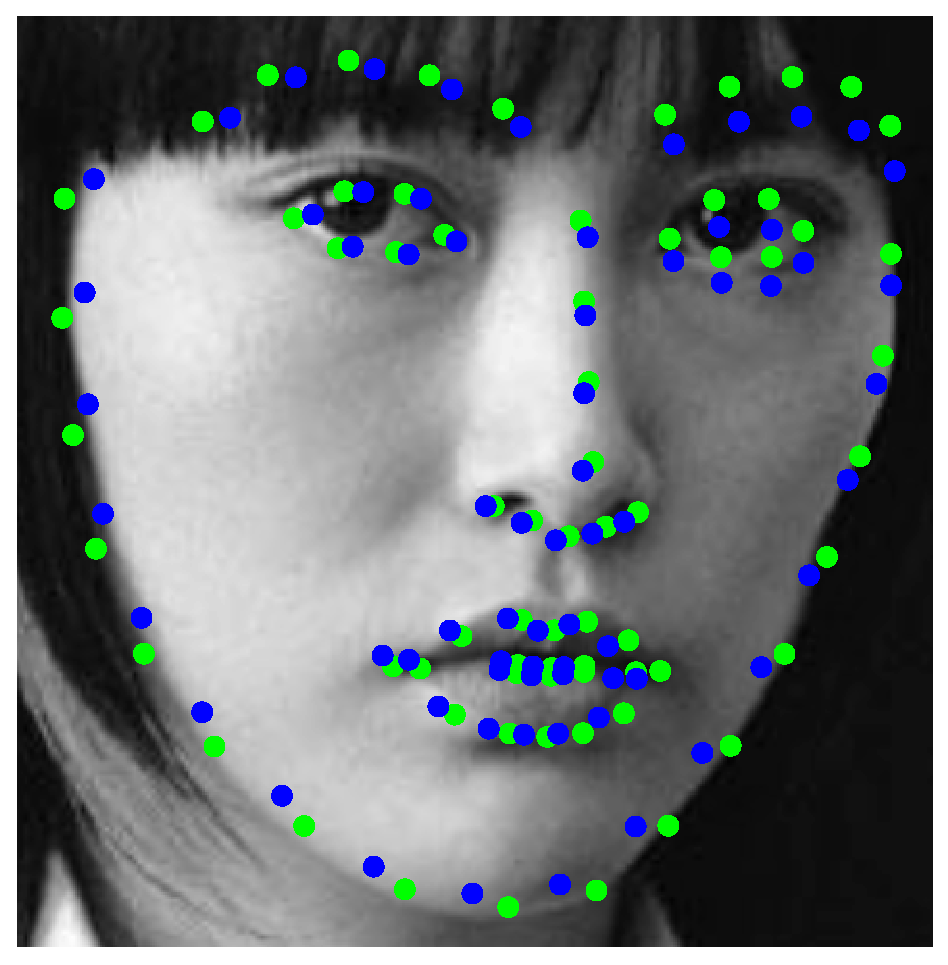
\includegraphics[height=\ofh]{face_all}
    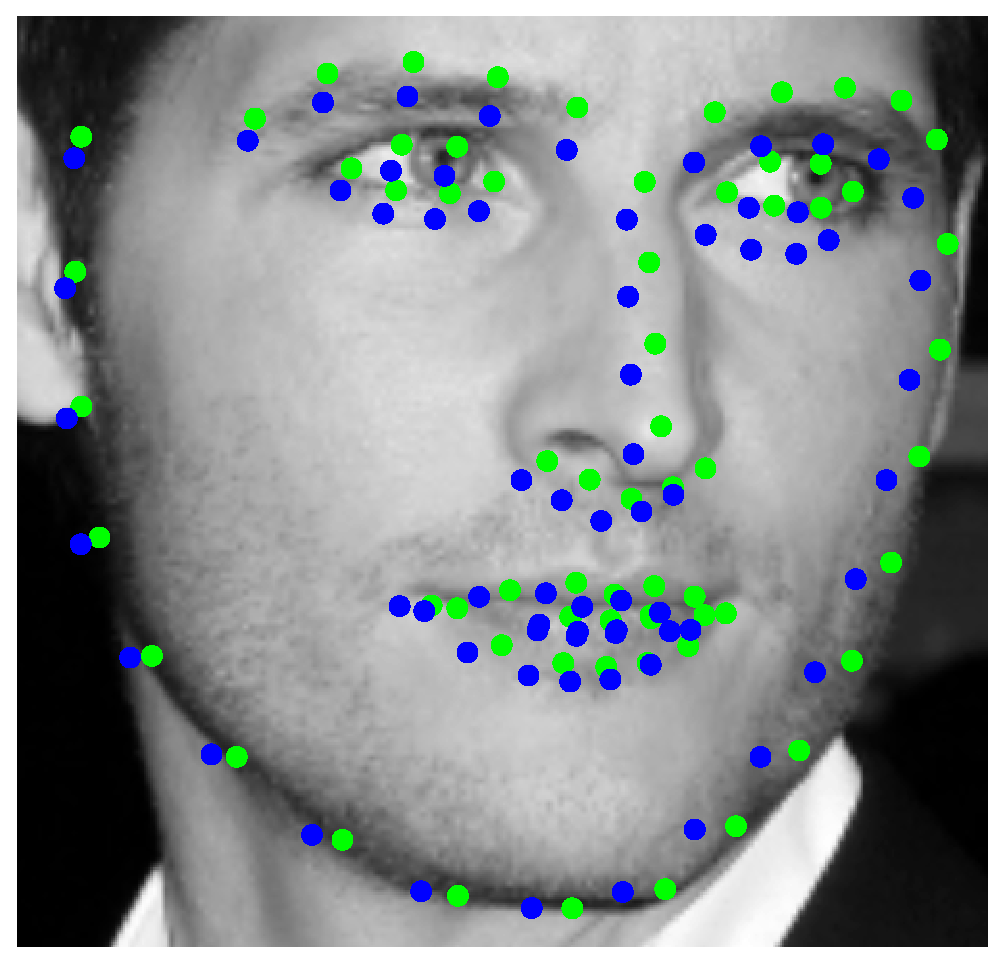
\includegraphics[height=\ofh]{face2_all}
    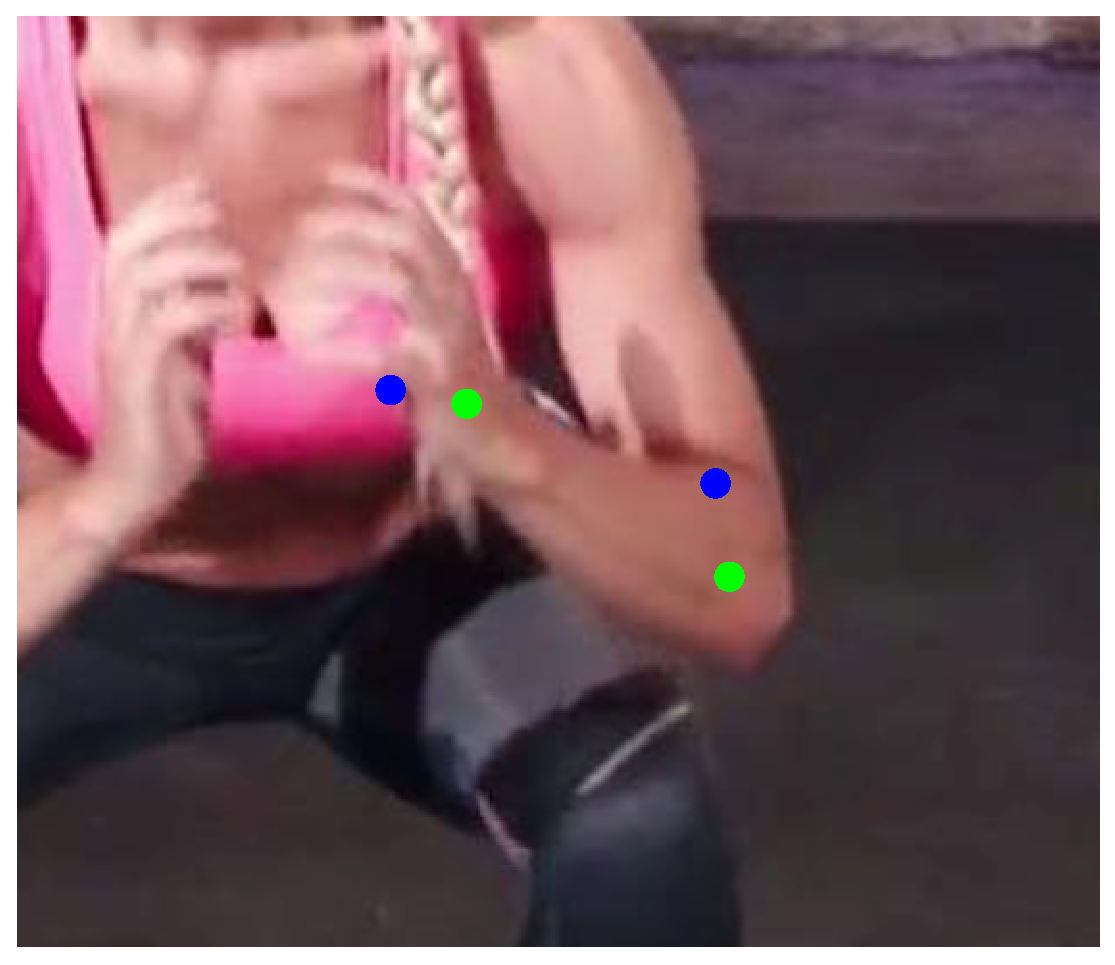
\includegraphics[height=\ofh]{arm_all}
    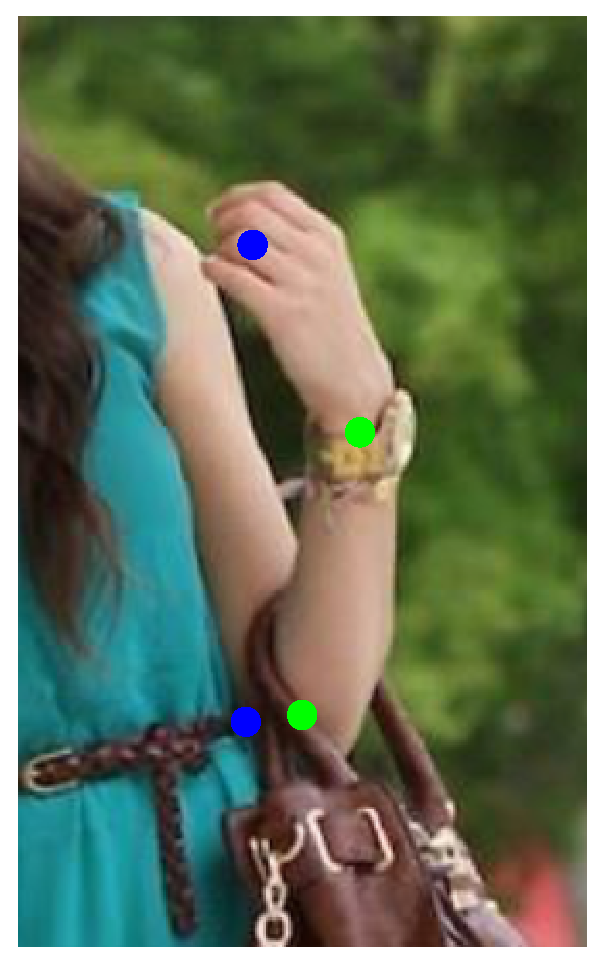
\includegraphics[height=\ofh]{arm2_all}
    \caption*{Figure A1. Visualisation of fitting models (faces and forearms) trained with noisy annotation (blue dots) and trained with consistent annotation (green dots).}
    \label{fig:noise_fitting}
    \vspace{-14pt}
\end{figure}


% LFPW EXPERIMENT
\textbf{[R23] Facial experiment on LFPW dataset.}
Unfortunately, LFPW database does not provide the actual images but only the original hyperlinks (from news-cites etc.) to them and currently most of them are inactive. We got the 224 from the authors of [24] who managed to download them 3 years ago. To keep it simple we have used state-of-the art AAMs such as [1,52] but on pixel intensities. State of the art includes the same methods but with image features such as HoGs [1,52] (in the revised paper, in Fig. 9, we will include AAMs on features).   

% PERFORMANCE ANALYSIS OF PROPOSED METHOD'S COMPONENTS
\textbf{[R23, R24, R25] Performance analysis of each component is missing. Difficult to implement.} 
Unfortunately, due to limited space we could not show the effect of all parameters involved in the pipeline. We plan to make such an analysis on a journal extension of this work. Nevertheless, we are committed to make the whole pipeline publicly available. 
% , as done with all software developed in our group,


\textbf{[R25] Full body model.} Currently, our aim, starting with arms, is to create contour models for each body part. Then, we are thinking of creating an articulated model that connects each of them, but this is future work on the topic. 

\textbf{[R25] Dimension of the $\mathbf{q}_i$ vector.} 
Every $\mathbf{q}_i$ is a sequence of 2D displacement vectors. It maps the image index $n$ ($n=1,..,N_t$ ) to a 2D vector 
$\mathbf{q}_i(n)$.  
Equivalently, $\mathbf{q}_i$ can be seen as a $2 N_t$ - dimensional vector, containing the displacements for all training images. 
%that correspond to the $i$-th basis element. 


 %We plan to make such an analysis on a journal extension of this work. We refer the %Reviewer to the relevant bibliography of each component (SVS [39], NICP [3], Flow %[27], dAAM [2], patch AAM [52]).


%\begin{figure}[t!]
%    \centering
%    \includegraphics[width=0.48\columnwidth]{noise2}
%    \caption{Benchmark between AAM trained with consistant and noisy data}
%    \label{fig:noise}
%\end{figure}






% \textbf{[R23, R25] Effort of complete contour annotation of the forearm}. In the case of forearm, taking only two points into account actually requires slightly more effort. But for usecase that requires more points, our pipeline will be much faster. Moreover, contour annotation can work with semantic segmentation which can make the pipeline fully automatic (boundary of semantic segmentation gives contours needed).



% \textbf{[R23, R25] Manual effort spent on obtaining richer annotation worth ... SDM can be built with less effort does not seem to apply to the lower arm model ... }




%{\small
%\bibliographystyle{ieee}
%\bibliography{bib}
%}

\end{document}
